% !TEX root = ../../Tesi_Triennale_PMNS.tex
\chapter[Osservazione di GW da BNS]{GW170817: osservazione di onde gravitazionali prodotte da un sistema binario di stelle di neutroni}
\label{chapter:gw170817}
Rivelato il 17 Agosto 2017 dal network LIGO-Virgo, GW170817 è il primo segnale di onda gravitazionale generato dallo spiraleggiamento un sistema binario di stelle di neutroni.
Il segnale osservato, alla fine del secondo run di misure O2, è tutt'ora il più energetico osservato finora tra questi tipi di segnale, con un rapporto segnale su rumore (SNR) di 32.4.

Oltre al segnale di GW è stato osservato un gamma ray burst, dopo 1.7s dalla coalescenza.
\section{Osservazione dello spiraleggiamento}
\label{section:osservazioneInspiralGW170817}
\begin{wrapfigure}{r}{0.5\textwidth}
	\vspace{-15pt}
	\begin{center}
		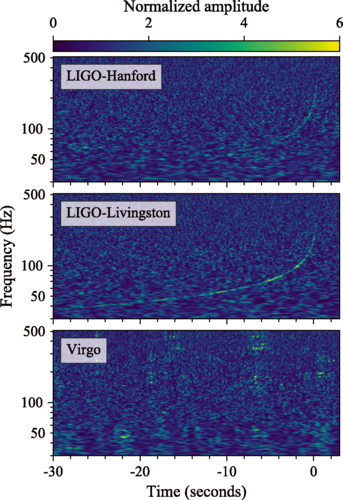
\includegraphics[width=0.4\textwidth]{figures/Capitolo_2/gw170817_time_freq.png}
	\end{center}
	\vspace{-10pt}
	\caption{Segnali in una mappa tempo frequenza nel network di detectors, presa da \cite{Abbott_2017b}}
	\label{fig:osservazione_gw170817}
	\vspace{-40pt}
\end{wrapfigure}
La rappresentazione tempo-frequenza dei dati a cui viene sottratto il rumore e sbiancati. Si può notare immediatamente che il segnale che, idealmente deve presentare la forma di un chirp, è ben visibile nei due rivelatori LIGO, meglio in Livingston che in Hanford, mentre in Virgo, a causa della posizione celeste della sorgente del segnale, non è possibile distiguere nessun pattern dal rumore di fondo. La (non) rivelazione risulta comunque utile, soprattutto per permettere l'individuazione della posizione celeste della sorgente.

L'analisi del segnale mostra un segnale coerente nei due detector LIGO, grazie al quale si individua la sorgente in una regione identificata da un angolo solido di 31 $\text{deg}^2$, che a sua volta ha permesso l'identificazione della controparte elettromagnetica GRB170817A. 
Si è ottenuto inoltre un SNR combinato tra i detector di 32.4 che rendono questo segnale il più intenso rivelato finora.\cite{Abbott_2017b}

\subsection{Proprietà della sorgente}
\label{subsection:proprietàSorgGW170817}
La relatività generale fa previsioni abbastanza dettagliate sull'evoluzione della frequenza, che è legato, nella prima fase, a una combinazione delle masse delle stelle progenitrici, detta massa di chirp 
\begin{equation}
	\mathcal{M} = \frac{(m_1m_2)^{3/5}}{(m_1+m_2)^{1/5}}
	\label{eqn:chirpmass}
\end{equation}
Nelle fasi più avanzate, le orbite si stringono e aumenta la frequenza dell'onda gravitazionale, mentre la fase della GW è sempre più influenzata da effetti relativistici legati al rapporto tra le masse $q = m_2/m_1$ e dagli accoppiamenti spin-orbita e spin-spin. 
La composizione interna degli oggetti diventa importante quando la distanza tra essi diventa paragonabile alle dimensioni dell'oggetto stesso. 

Le proprietà della sorgente di onde gravitazionali sono ottenute dal confronto con le forme d'onda predette dalla teoria. Viene fatta dunque una analisi Bayesiana nel range di frequenze 30-2048Hz che include gli effetti dell'incertezza di calibrazione di $1\sigma$ sul segnale ricevuto.

La sorgente viene in questo modo identificata in una regione celeste di 28$\text{deg}^2$ di area e $380\text{Mpc}^3$ di volume, utilizzando una combinazione di timing, fase e ampiezza dei tre detector. La distanza luminosa, la più prossima osservata finora, viene individuata in $40_{-14}^{+8}$Mpc. Per le masse delle stelle compatte risulta più semplice dedurre la massa di chirp, indipendente dalla scelta della prior nell'analisi Bayesiana, che si valuta in $\mathcal{M}=1.188_{-0.002}^{+0.004}$, rispetto alle masse singole, che soffrono invece della degenerazione tra il rapporto tra le masse $q$ e le componenti dello spin $\chi_1$ e $\chi_2$. È necessario fare quindi assunzioni a partire dalle EOS che si considerano, ottenendo dei range $m_1 \in (1.36, 2.26)M_\odot$ e $m_2 \in (0.86, 1.36)M_\odot$ evidentemente meno precisi, ma comunque utili come evidenza della natura di stelle di neutroni del sistema binario, escludendo invece la possibilità di buchi neri che prevederebbe range di masse superiori\cite{Abbott_2017b}.

QUALCOSA SULLE TIDAL DEFORMABILITIES?
\section{Ricerca del post-merger del residuo}
\label{section:postmergerGW170817}
L'analisi del post-merger, atteso in seguito all'osservazione del segnale GW170817, non ha portato ad evidenza statisticamente significativa di un oggetto in seguito alla coalescenza, ma ha permesso di ottenere informazioni sul limite superiore sulle ampiezze di strain ed energie di GW osservabili. Gli attuali detector infatti non sono calibrati in modo tale da permettere rivelazioni alle alte frequenze del post-merger.

Mentre lo studio del segnale elettromagnetico associato alla GW non permette di escludere nessuno dei possibili stati finali indicati in sezione \ref{section:residual}, grazie ai valori ottenuti per le masse dei progenitori date nella sezione \ref{subsection:proprietàSorgGW170817} si calcola che per un ampio range di equazioni di stato la coalescenza produce uno stato di NS ipermassiva. Questo spiega anche il ritardo del lampo-$\gamma$rispetto all'istante di rivelazione del segnale di merger. 

\begin{wrapfigure}{r}{0.5\textwidth}
	\vspace{-15pt}
	\begin{center}
		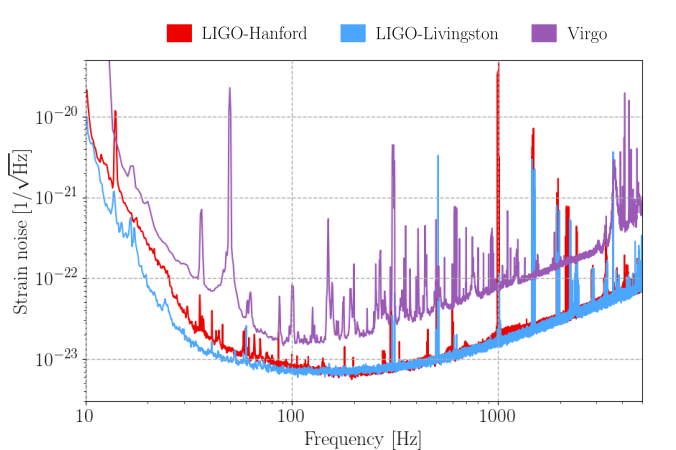
\includegraphics[width=0.5\textwidth]{figures/Capitolo_2/noiseData.png}
	\end{center}
	\vspace{-5pt}
	\caption{Sensibilità di ciascun rivelatore durante il run O2, indicata dall'ampiezza del rumore di strain in funzione della frequenza, presa da \cite{Abbott_2019}}
	\label{fig:NoiseFrequenze}
	\vspace{-10pt}
\end{wrapfigure}
Come si vedrà nella sezione \ref{section:analisiSimSingole} in base alla EOS che si considera si ottiene un contributo diverso nel post-merger che inizia attorno a $\smallsim1$kHz. Più in generale, oltre alla EOS hanno fondamentale importanza le masse e gli spin degli oggetti iniziali. 
Per quanto riguarda invece la rivelazione di questa fase del segnale, anche considerando modelli ottimistici da stati finali di NS ipermassiva o supermassiva, l'SNR atteso per distanze di $\smallsim40$Mpc è $\smallsim1-2$ ordini di grandezza più piccolo di quello rivelabile dal network LIGO-Virgo attualmente utilizzato, facendo uso di algoritmi di confronto con segnali modellati (che comunque sono meno utilizzati per il post-merger, per la difficoltà nel modellare questa fase del segnale).
Si ipotizza tuttavia che nei prossimi run O3-O4 la sensibilità del network sarà tale da permettere la rivelazione di queste emissioni.

Come si può osservare in figura \ref{fig:NoiseFrequenze} i tre detector del network hanno zone diverse di sensibilità, in particolare si nota che in generale la sensibilità diminuisce significativamente ad alte frequenze. Il rumore di LIGO Hanford è più alto rispetto a Livingston nella banda di frequenza compresa tra 100Hz e 1kHz, mentre Virgo ha sofferto grandi fluttuazioni di rumore e proprietà spettrali non stazionarie a frequenze superiori a 2.5kHz.

Per l'analisi sono stati usati due diversi algoritmi, in base al tipo di segnale ricercato: per segnali di brave durata è stato usato cWB (Coherent Wave Burst) utilizzando i dati di LIGO tra 1024Hz e 4096Hz, mentre per i segnali di durata intermedia si è utilizzato l'algoritmo STAMP (Stochastic Transient Analysis Multidetector Pipeline) nelle frequenze comprese tra 24Hz e 2000Hz e tra 2000Hz e 4000Hz nei dati di LIGO, mentre cWB con i dati del network LIGO-Virgo ricerca le frequenze tra 24Hz e 2048Hz. 

Per la ricerca di segnali con incertezze teoriche cosi grandi l'utilizzo di metodi di ricerca matched-filtering, ovvero un metodo che utilizza segnali di forme conosciute e attraverso funzioni di filtraggio si esclude la componente di rumore, in particolare si sceglie la funzione che massimizza il rapporto segnale su rumore (SNR) per tale segnale\cite{maggiore2008gravitational}. È immediato comprendere che non conoscendo con certezza la forma che deve assumere il segnale questo metodo risulta inefficace per la ricerca del post-merger. Gli algoritmi che si usano ricercano eccessi di potenza in una mappa tempo-frequenza e usando metodi di riconoscimento dei pattern si può identificare la presenza di segnali di GW nelle mappe. In particolare gli algoritmi sono tali da considerare i dati del network e non dei singoli rivelatori, utilizzando tecniche che permettono di combinare coerentemente i dati dei singoli detector e dare risposte differenti a forme d'onda diverse.

Come anticipato, la ricerca viene divisa tra segnali brevi ($\lesssim$1s) e intermedi ($\lesssim$500s).
\subsection{Segnali brevi}
L'analisi dei segnali brevi, ad alte frequenze viene fatta con l'algoritmo cWB e consistono nella ricerca di eccessi di potenza nell'intervallo di 2s che precede il segnale elettromagnetico GRB 170817a, che comprende quindi anche il merger.
In particolare l'algoritmo valuta la massima verosimiglianza di eccessi di potenza in una trasformata di wavelet a multi-risoluzione per ogni detector, classificando gli eventi in una gerarchia di SNR. La significanza degli eventi è data dal confronto con la distribuzione del fondo stocastico, che è generata con metodi che saranno precisati nel capitolo \ref{chapter:cwb}. 

È convenzione esprimere la sensibilità della ricerca di una data forma d'onda in $h_{rss}^{50\%}$, ovvero la somma in quadratura delle ampiezze di strain di segnali che sono rivelati con un'efficienza del 50\%. La quantità $h_{rss}$ è definito come
\begin{equation}
	h_{rss} = \sqrt{2\int_{f_{min}}^{f_{max}}df(|\tilde{h}_+(f)|^2 + |\tilde{h}_\times(f)|^2 )}
\end{equation}
dove $f_{min}$ e $f_{max}$ sono rispettivamente le frequenze massima e minima sulle quali si effettua la ricerca. 
Il criterio su $h_{rss}^{50\%}$ scelto per questo metodo di ricerca è tale da avere una probabilità di falso allarme di $10^{-4}$

Per evitare la possibile perdita di segnali di EOS rigide, si fa la scelta conservativa di ricercare segnali a partire da 1024Hz, nonostante tutte le forme d'onda hanno emissioni dominanti molto al di sopra di tale soglia.

In conclusione, non viene trovata evidenza di nessun segnale di GW in questa banda di frequenze.
L'ampiezza di strain per produrre una probabilità del 50\% di rivelazione di un segnale è compresa tra $2.1 x 10^{-22} \text{Hz}^{-1/2}$ e $3.5 x 10^{-22} \text{Hz}^{-1/2}$. L'energia irradiata da un sorgente che emette isotropicamente è data da 
\begin{equation}
	E_{gw}^{iso} = \frac{\pi c^3}{2G}\mathcal{D}^2\int d\Omega \int_{f_{min}}^{f_{max}}dff^2(|\tilde{h}_+(f)|^2 + |\tilde{h}_\times(f)|^2 ) \approx \frac{\pi^2 c^3}{G}\mathcal{D}^2\bar{f}^2h_{rss}^2
\end{equation}
con $\mathcal{D}$ è la distanza dalla sorgente e $\bar{f}$ è la frequenza caratteristica data da 
\begin{equation}
	\bar{f} = \frac{2}{h_{rss}^2}\int_{f_{min}}^{f_{max}}dff(|\tilde{h}_+(f)|^2 + |\tilde{h}_\times(f)|^2 )
\end{equation}

In questo modo si ottiene un range di energie rivelabili secondo il criterio del $h_{rss}^{500\%}$ è dato da $4.8-\SI{19.6}{\solarmass}c^2$, al di fuori delle masse in gioco per BNS, per cui non è possibile con i rivelatori attuali rivelare le emissioni di GW di NS ipermassive associate a GW170817.
\subsection{Segnali di durata intermedia}
Per segnali di durata intermedia si utilizzano i due algoritmi cWB e STAMP, concentrando la ricerca in una zona limitata dello spazio, indicata dalla controparte elettromagnetica che permette di evitare trigger accidentali.

\begin{wrapfigure}{r}{0.5\textwidth}
	\vspace{-15pt}
	\begin{center}
		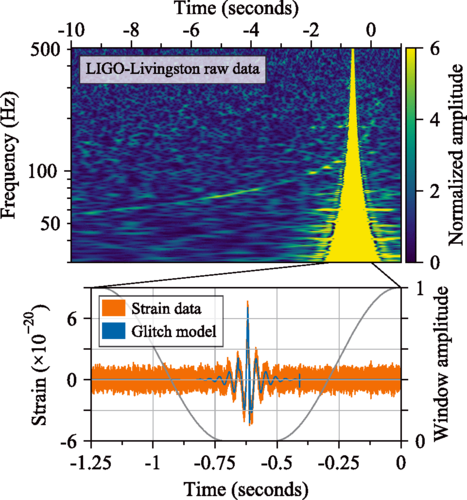
\includegraphics[width=0.5\textwidth]{figures/Capitolo_2/signal.png}
	\end{center}
	\vspace{-5pt}
	\caption{\cite{Abbott_2017b}}
	\label{fig:signalInspiral}
	\vspace{-10pt}
\end{wrapfigure}
\section{Sugli altri eventi rivelati}
\subsection*{title}
%Breve rassegna dei metodi di rivelazione: stamp \& cwb

non trovato alcun segnale\cite{Abbott_2017a}